\section{Understanding errors and getting help}
\label{sec:errors}

Even though re-using code makes writing programs easier and less error-prone, of course you will make errors. 
Programming can be a frustrating endeavour, and you will encounter error messages, bugs, and problems that you don’t know how to fix. This section shows how error messages are useful rather than scary and lists the main error messages encountered in the beginning. It explains how to search for help within the R/Python documentation, how to use online resources, and how to formulate questions to your instructor or community so you get a useful answer. 

If you tried out some of the concepts in \refchap{programmingconcepts}, you have probably already come across some typical or basic errors in programming. Maybe you tried to call a function from a library that you forgot to load before, or maybe you tried to multiply a string with a float.
There are thousands of more errors that you will encounter, and there is no extensive list of them, so you won't find a complete structured catalogue to solve your problems when coding. This might seem a rough road for any scientist but in fact you will get used to find the answers by different means.

\subsection{Error messages}


There are two common strategies to \textit{avoid getting stuck} and move on with your task: one is to understand the \textit{type} of error you are getting, and the other is to know \textit{where} to go to obtain valuable help. We would add a third one: be patient and do not despair!

Both R and Python produce warning or error messages when something is wrong in your code. Beginning computational researchers may sometimes feel afraid, confused, or even frustrated when they get such a \textit{painful} message (we have all felt it actually) and some then would become so anxious that they won't pay enough attention to the text of the error message thinking it will not be helpful to solve the problem and blaming themselves for not being a perfect programmer. But the more you code the more your realize that getting this error messages is just part of the routine and that it is highly useful to carefully read the warning instead of skip it.

In most cases, the error message in your console will tell where exactly the problem is: a specific line or operation within your code. With this information in many cases you will quickly identify what the problem is about and you will know how to solve it. One of the most common causes for an error are just very silly typo's!

Next to the location (the line number), the error message will also tell more about the problem. For example, when trying to multiply the float object \texttt{a} by the string object \texttt{b} you will get ``Error in a * b : non-numeric argument to binary operator'' in R or ``TypeError: can't multiply sequence by non-int of type 'float' '' in Python. As intimidating as this language may sound in the first place, if you re-read it, you will realise that they, in fact, explain exactly what went wrong. This helps you to understand what you did wrong and enable you to fix it. 

% I (Damian) commented out the part about compile time and runtime errors, because (a) it may be confusing as both are interpreted languages [OK Python code is compiled into bytecode but all of that is pretty complicated], and (b) because I think it doesn't really matter for beginners

%Theoretically, there are different types of errors that may arise: \texttt{syntax} (incorrect syntax of the code such as missing the final parenthesis), \texttt{semantic} (incorrect use of program statements such as computing an operation you don't really need or want) and \texttt{logical} (incorrect use of program flow such as use a wrong conditional operator). In the case of syntax errors the compiler will detect them, but not always in the case of semantic and logical. Specifically, when R or Python detects and alert of an error we well call them \texttt{compile time errors} and will include syntax and \textit{static} semantic errors. When the compilers do not alert we will call them \texttt{runtime errors} and include logical and \textit{dynamic} semantic errors.

%You do not really have to care much about the typology of errors now, but at this point we encourage you to solve them by yourself or to ask for help in the proper terms.

If you get a warning error that don't understand or get an incorrect result in your code you have three options before getting stuck: use the \texttt{help} commands to know more about any object or function (\verb|help(object)| in both R and  Python); read the documentation of base R, base Python or of any individual package (there are plenty of them online!); and look at the wonderful community of worldwide coders, read what they have discussed so far or even pose a question to \textit{challenge} their minds.

Let's discuss a little bit this last third option. Imagine you read the text of an error message and you feel you don't understand it. It may be because the wording is too complex or because it just gives an ``error code'' (i.e. ``error 401 - Unauthorized'' when trying to connect to the Twitter API). If you think of searching for it in Google, your first choice is completely correct: it might take you to code documentation, or better to an online discussion in sites such as Stack Overflow, which is a useful question and answer website for coders (see Figure~\ref{fig:stackover}). It is very likely that some colleagues had already posed a question about the meaning of that error and others have already answered what it means and especially \textit{how to} fix it. In fact, you will also find many questions refereed of \textit{how to} perform different tasks in R or Python (and in many other languages!),  making this kind of sites valuable repositories that will help you to solve your daily problems.

\begin{figure}
\centering
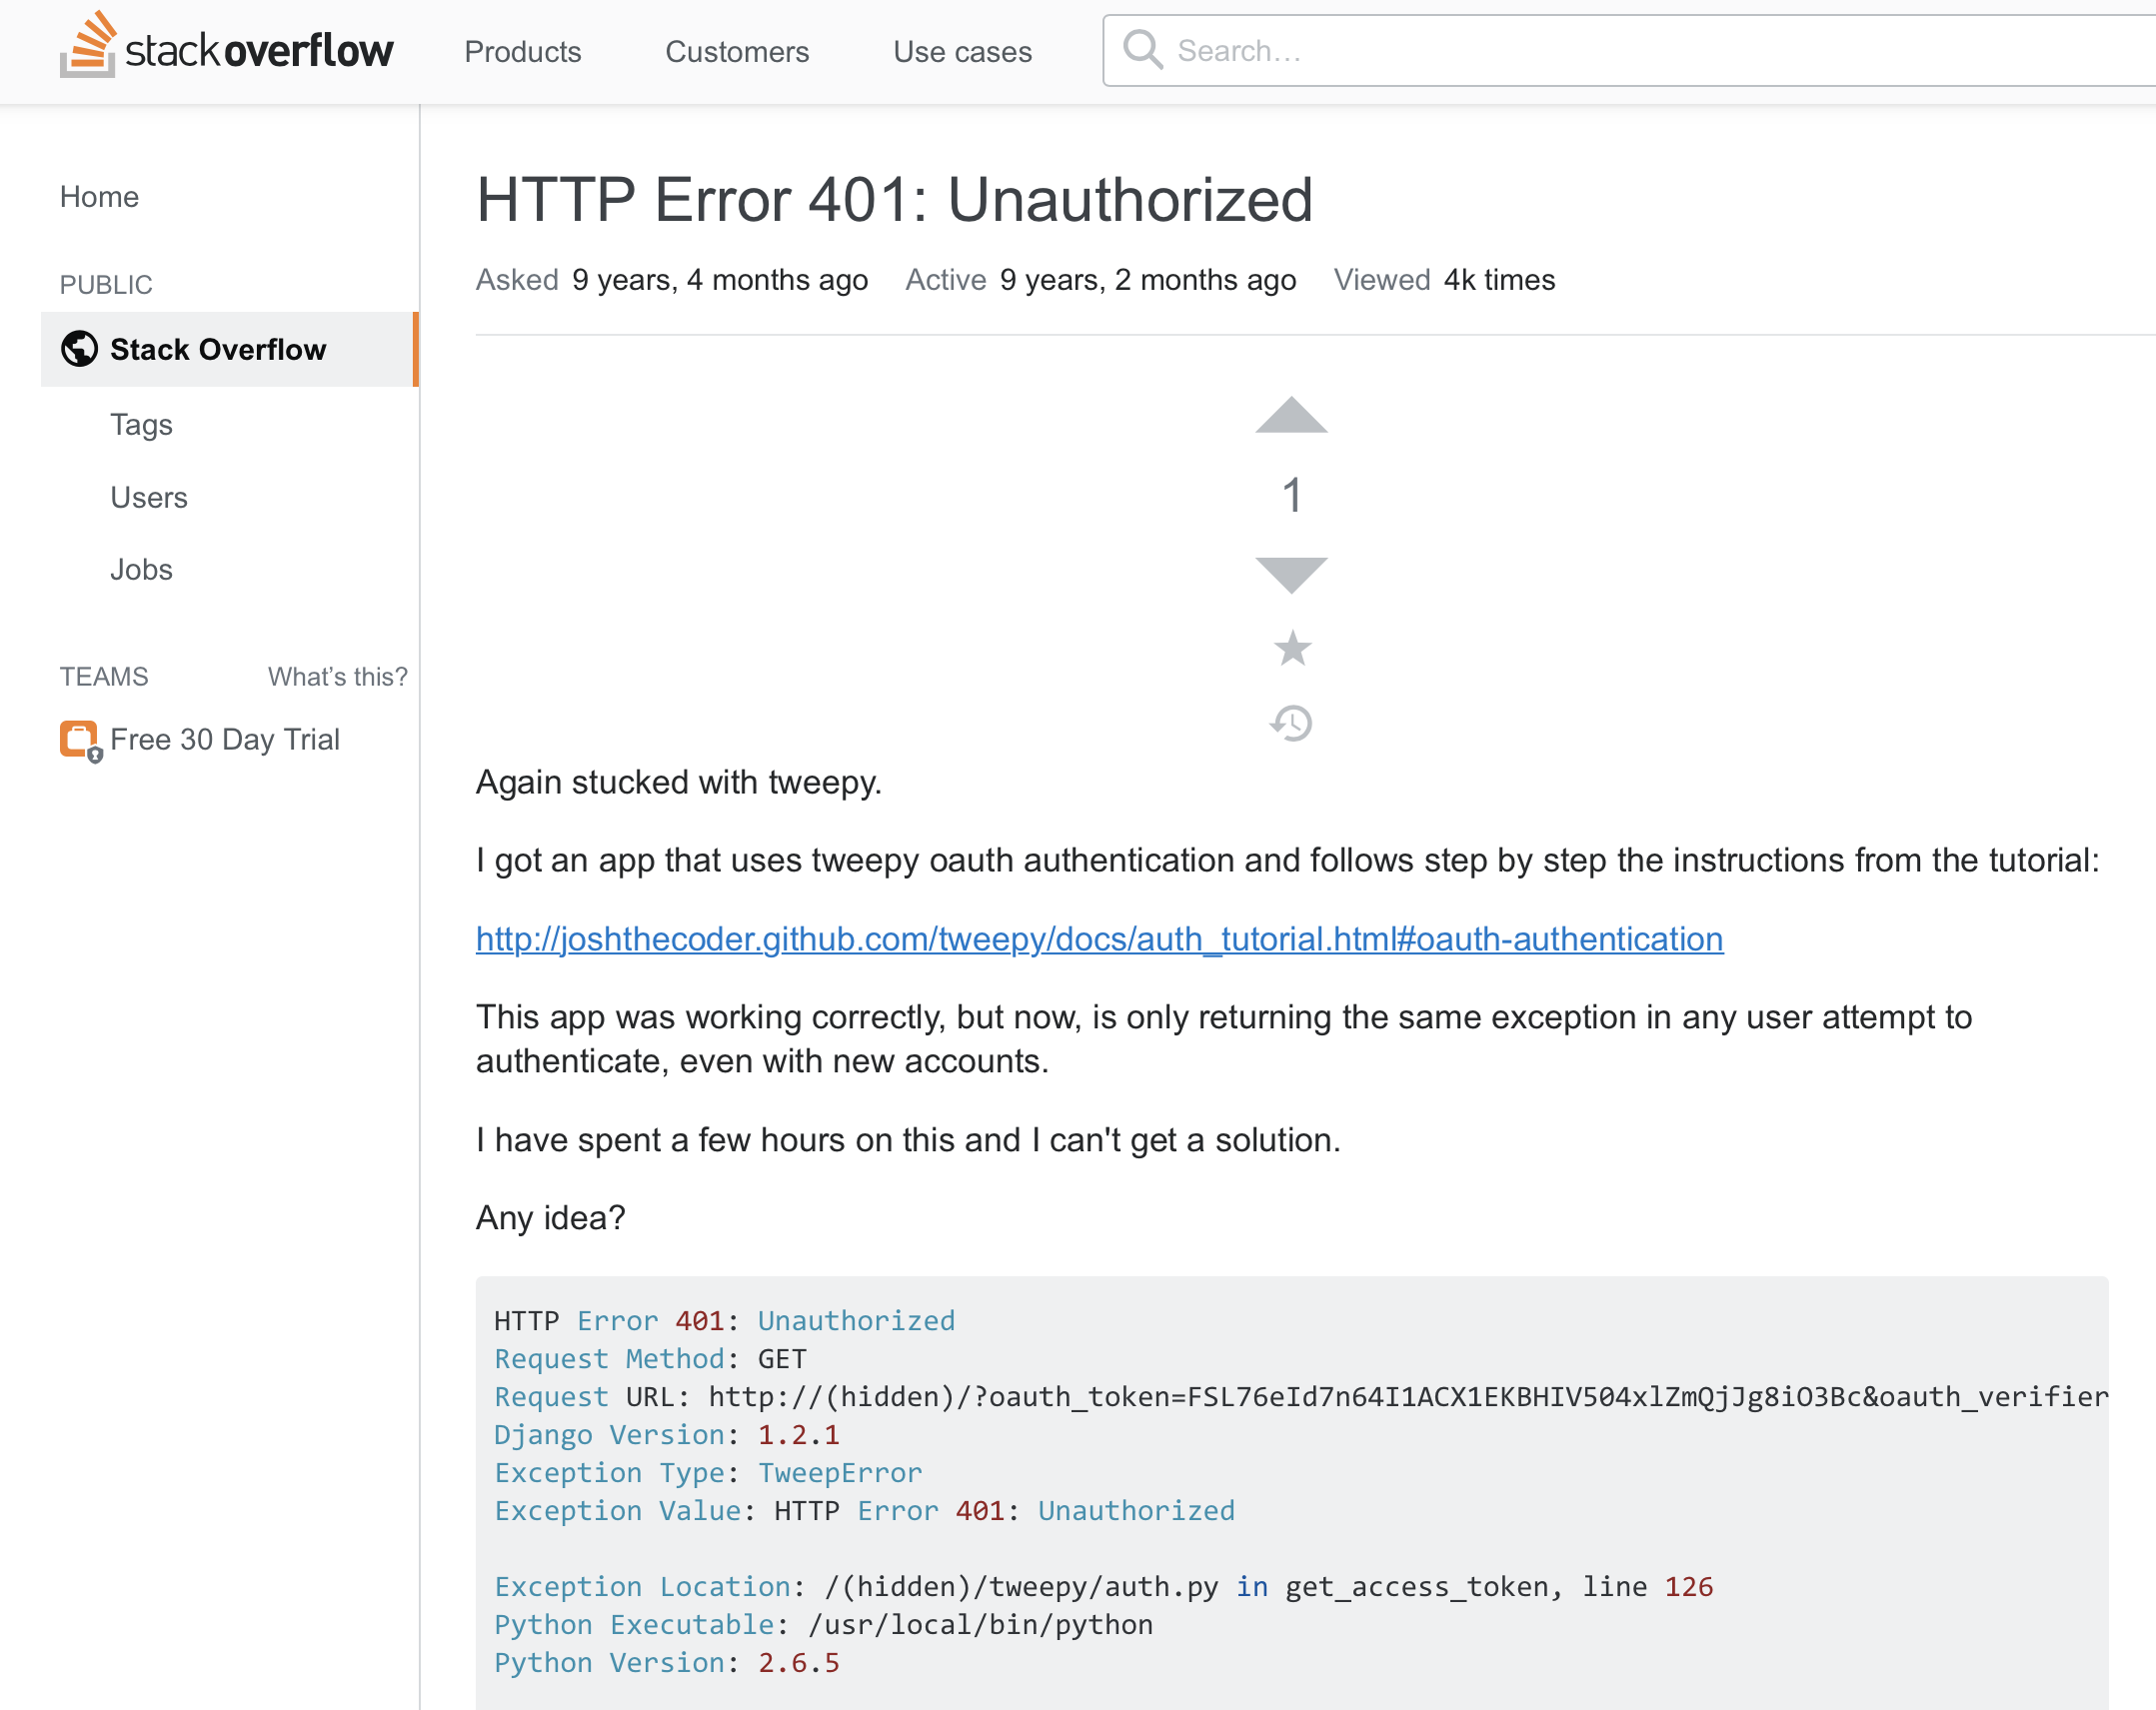
\includegraphics[width=0.9\linewidth]{figures/ch4_stackover}
\caption{A online discussion in Stackover Flow about a warning message }
\label{fig:stackover}
\end{figure}

Depending on the complexity and novelty of your problem you will find a helpful answer in few minutes or it might take you hours. Never get desperate if you visit many discussions without getting what you look at once: you may have to come back to some of them after reading all. Moreover, some answers will include the exact code you need (ready for copy-and-paste), code to be adapted (i.e. changing the name of your variables) or in pseudocode (informal description of the code). In all of the cases you will be the responsible for making sense of the huge (and sometimes messy) amount of sources you will come across. 

It is of course possible that you don't get what you need in previous discussions. For that you will be able to create your own question and wait for anyone to reply. If you decide to do this, take some advices into account. First, be sure that the answer is not elsewhere within the same website (a first answer could be just a link to a previous post!). Second, don't be afraid thinking that your question is silly or too basic: you will find in the community all kind of coders, from those who are taking their first steps to those advanced. Third, be clear, concrete and focus on what you need too solve. This is probably the most important advice since it is necessary that other coders quickly understand what you need in few words (not philosophical discussions or previous elaborated rationales) and so they can decide to spend some minutes of their time and help you. It is a very common practice that you copy in the questions the warning message or the code you are having trouble with because peers can even fix it themselves and give the solution right away. Do not worry if your post receives a lot of replies after getting what you needed. This thread might also help others in the future!


\subsection{Debugging strategies}

It's not always equally straightforward to see what is going
wrong. Maybe your script does not even produce an error
message, but just produces some unexpected result.

Of course, every program is different and there is not one
way to solve every issue, but there are some simple strategies
that help you debugging your code. The underlying core
principle is to better understand what exactly is happening.

\begin{itemize}
  \item Print more. For example, if you have a for-loop, just add a print statement to the loop that prints the current value that is processed, or some other information that helps you understanding what data exactly are processed, or what intermediate result is achieved at which step There are more advanced tools for keeping track of values, such as so-called \concept{debugger}s in advanced IDEs or the \pkg{logging} module in Python, but a couple of extra print functions can serve the same purpose.
  \item Keep track of which code blocks have been executed how often. For instance, maybe you have some if statement, but the condition is simply never True, so that the whole code block is never executed. You can create an integer with value 0 at the beginning of the code, and then increment it by one within the code block. If you print it afterwards, you know how often the block has been visited.
  \item Cut it down. Remove (comment out) everything that is not strictly neccessary and see whether you can make a simplified version of your code run, before you extend it.
  \item Add consistency checks. For instance, if from a theoretical point of view, two lists need to have the same length, check it with the length function; similarly, if you know that an object must have a specific value (e.g., because you know the result), check this assumption.
\end{itemize}


Finally, when you know that some typical errors may arise and you don't want your script to stop or crash, you can add an \texttt{exception} in your code. Imagine for example to build a function to connect to any API (see Section \refsec{apis}). There might be many reasons for getting an error and then stops the script (such an internet disconnection!). You might decide to skip  the error and continue the next lines or even you can give a more detail instructions of what to do (i.e. wait 5 minutes and try again). The inclusion of these exceptions are in fact a good practice and will help your code to be more robust and stable.

Let's make \refex{if1} from the previous chapter more robust so that it does not fail if an invalid headline is passed. For instance, in Python, the object |None| has no defined length; and in R, it is illegal to calcuate the number of characters in a factor. It is a good idea to think about how you want to deal with this: either you want your script to just fail (and clean up the data), or you may want to deal with the error in some way. Especially if you have little control over the input data and/or if the process you are dealing with takes a long time, you may want to rather handle these errors instead of having your script fail. In \refex{tryexcept}, we show how to use such a try/except construction: you indicate which code block you want to try (e.g., run as normal); and in the next block, you indicate what should happen if that results in an error.

Note that using \concept{try .. except} statements like this is fairly common in Python code,
but in R it is usually not needed as in many cases where a Python function like \verb|int| raises and exception
if the input cannot be converted to an integer, while the R function \verb|as.numeric| returns a missing value.
Thus, in R you normally only encounter these statements when using external resources,
for example when using an API or scraping a webpage. See \refchap{scraping} for more details on these topics. 

\pyrex[input=both,output=both,caption={Error handling.}]{chapter04/tryexcept}
